\chapter{In litterae}


\section{Trwałość amidów}

\begin{marginfigure}[7\baselineskip]
  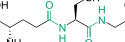
\includegraphics{schemes/glutathione}
  \caption{
    Glutation \--- trójpeptyd o~właściwościach przeciwulteniających,
    z~wiązaniami amidowymi zanaczonumi na~zielono.
  }
  \label{fig:glutathione}
\end{marginfigure}
Wiązanie amidowe występuje w~naturze niezwykle powszechnie.
Można nawet pokusić się o~stwierdzenie, że jest ono jednym z~budulców życia \---
w~końcu peptydy, podstawowa struktura biocheniczna złożonych organizmów,
to łańcuchy aminowkasów, połączonych wiązaniami amidowymi.
Za~przykład posłużyć może glutation \--- trójpeptyd o~właściwościach przeciwulteniających,
występujący powszechnie w~organizmach roślinnych i~zwierzęcych\autocite{wu04},
przedstawiony na~\cref{fig:glutathione}.
  
\begin{marginfigure}
  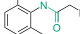
\includegraphics{schemes/lidocaine}
  \caption{
    Lidokaina \--- przykład leku posiadającego ugrupowanie amidowe
    (zaznaczone na~zielono).
  }
  \label{fig:lidocaine}
\end{marginfigure}
Ugrupowanie to~można też znaleźć w~wielu związkach biologicznie czynnych.
Za~prosty przykład niech posłuży lidokaina, przedstawiona na~\cref{fig:lidocaine},
powszechnie stosowana jako środek miejscowo znieczulający.
Przykładów takich możnaby przytoczyć wiele, bo~jak pokazuje analiza produkcji farmaceutyków,
\SI{66}{\percent} leków syntezuje się tworząc wiązanie amidowe\autocite{carey06}.

W~latach 30. ubiegłego wieku firma DuPont wprowadziła na~rynek poliamidy na~rynek tworzyw sztucznych pod nazwą handlową Nylon.
Ten bardzo trwały materiał szybko znalazł zastosowanie w~wielu gałęziach przemysłu.
Stosuje się go przede wszystkim do~wytwarzania syntetycznych włókien tekstylnych,
ale też do~produkcji szczoteczek do~zębów, strun do~instrumentów, żyłek wędkarskich, czy opakowań żywności.

Tę powszechność \--- zarówno wśród produktów naturalnych, jak i~wytworów cywilizacji \---
amidy zawdzięczają między innymi swojej wyjątkowo niskiej reaktywności względem innych karbonyli.
Dobrze obrazuje to liniowa skala karbonylowości zaproponowana przez Mucsiego i Chassa (\cref{fig:carbonyl-scale})\autocite{mucsi08}.
Wiązanie amidowe ulega niewielu przemianom chemicznym, a~jeśli już, to~
zwykle wymaga stosowania bardzo ostrych warunków prowadzenia reakcji.
Ta niezwykła trwałosć wynika z~bardzo efentywnego nakładania się orbitali 
molekularnych atomu azotu oraz $\pi$ wiązania podwójnego \ch{C=O}.
Pozwala to na~wydajną delokalizację elektronów w~obrębie wiązania i~znaczny 
udział dwóch możliwych struktur dipolarnych, jak widać na~\cref{sch:resonance}.
\begin{marginscheme}
  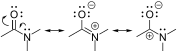
\includegraphics{schemes/resonance}
  \caption{
    Struktury rezonansowe wiązania amidowego, zapewniające mu~niezwykłą trwałość.
  }
  \label{sch:resonance}
\end{marginscheme}

\begin{figure}
  \centering
  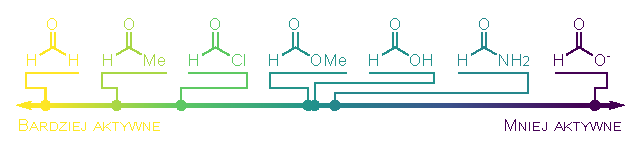
\includegraphics{schemes/carbonyl-scale-acc}
  \caption{
    Względna reaktywność róźnych grup karbonylowych
    wg skali karbonylowości Mucsiego i Chassa.
  }
  \label{fig:carbonyl-scale}
\end{figure}


\section{Prezkształcenia amidów}
Już w~drugiej połowie XIX~w. chemicy wiedzieli, że pierwszorzędowe amidy mogą ulegać reakcji odwodnienia, dając nitryle.
W~roku \citeyear{wallach77} udało się po raz pierwszy przeprowadzić taką reakcję na amidach drugorzędowych\autocite{wallach77}.
\citeauthor{wallach77} dokonał tego stosując \ch{PCl5} jako reagent.
To doniesienie jest pierwszą publikacją na temat przekształceń amidów, jakią można znaleźć w~literaturze.
\todo{Dodać przegrupowanie Hoffmanna}
\begin{marginscheme}
  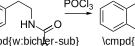
\includegraphics{schemes/bichler}
  \caption{Ogólny schemat reakcji Bichlera-Napieralskiego.}
  \label{sch:bichler}
\end{marginscheme}
W~\citeyear{bischler93} \citeauthor{bischler93} pokazali, że działając \ch{POCl3}
na~amid wywiedziony z~\iupac{2-fenyloetyloaminy} można otrzymać pochodną dihydroizochinoliny\autocite{bischler93}.
Jakiś czas później wariację tej przemiany przedstawili \citeauthor{pictet10}.
Wychodząc z~\iupac{2-hydroksy-2-fenetyloamidu} otrzymali w jednym etapie produkt już odwodniony \--- izochinolinę\autocite{pictet10}.
W~roku \citeyear{vilsmeier27} \citeauthor{vilsmeier27} pokazali, że reakcję tę można prowadzić nie tylko wewnątrzcząsteczkowo;
nie da się jednak zatrzymać jej na~etapie addycji do~arenu.
Realcja \iupac{\N,\,\N-dimetyloamidu} z~\ch{POCl3} prowadzi do~powstania kationu chloroiminiowego, nazywanego też reagentem Vilsmeiera.
Ulega on addycji do bogatych w elektrony arenów, tworząc iminę.
Podczas przerobu reakcji następuje hydroliza tego adduktu, skutkując powstaniem odpowiedniego aldehydu (lub ketonu) arylowego\autocite{vilsmeier27}.
\begin{scheme}
  \centering
  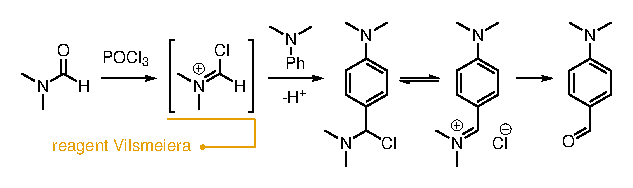
\includegraphics{schemes/vilsmeier}
  \caption{Mechanizm reakcji Vismeiera-Haacka.}
  \label{sch:vilsmeier}
  \setfloatalignment{b}
\end{scheme}

Dopiero w~roku \citeyear{brown48} pojawiła się w~literaturze wzmianka o~syntezie amin z~amidów.\todo{poprawić po dodaniu Hoffmanna}
\citeauthor{brown48} pokazali, że możliwa jest redukcja amidowej grupy karbonylowej za pomocą glinowodorku litu\autocite{brown48}.
Reakcja ta jest dzisiaj chyba najbardziej sztandarowym przykładem reaktywności amidów.
Razem z~reakcją odwodnienia, hydrolizą, oraz reakcjami Vilsmeiera-Haacka i~Bischlera-Napieralskiego,
stanowi teraz podręcznikowy kanon.
Przez długi czas przemiany te były właściwie jedynymi dostępnymi chemikom metodami modyfikacji grupy amidowej.
Wszystkie wymagały użycia agresywnych warunków,
które z~dużym prawdopodobieństwem byłyby niekompatybilne z~innymi grupami funkcyjnymi obecnymi w~związku.
Chemia amidów była więc raczej uboga, a~wykorzystanie wiązania amidowego w~syntezie często sprowadzało się do jego obecności w~produktach.

Przełomem w~tej materii była praca, którą opublikowali \citeauthor{ghosez69} w~\citeyear{ghosez69} roku.
Przedstawili oni metodę syntezy \iupac{\a-chloro enamin} z~amidów przy użyciu fosgenu i zasady (trietyloaminy lub pirydyny)\autocite{ghosez69}.
Autorzy byli zaskoczeni łatwością z~jaką związki te ulegają nukleofilowej substytucji atomu chloru.
W roli nukleofila przetestowali reagenty Grignarda, związki litoorganiczne, alkoholany, tiolany araz amidki
(oznaczone na \cref{sch:chloroenamine} ogólnie jako \ch{Nu-}),
otrzymując produkty z~dobrymi wydajnościami (\SIrange{65}{90}{\percent}).
Publikacja ta rozpoczyna nową erę w chemii amidów, dając początek idei \emph{aktywacji wiązania amidowego}.
\begin{scheme}
  \centering
  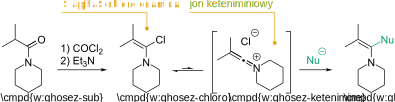
\includegraphics{schemes/chloroenamine}
  \caption{Aktywacja amidu przez przekształcenie w \iupac{\a-chloro} enaminę.}
  \label{sch:chloroenamine}
\end{scheme}


\section{Aktywatory tryflowe}
% W przeciwieństwie do ketenów, sole keteniminiowe ulegają formalnej [2+2] cykloaddycji alkenów i~alkinów
Gdy metodologia zaprezentowana przez Ghoseza i~in. została dokładniej przetestowana, okazało się że nie jest wolna od wad \---
wyzwaniem jest wykorzystanie soli keteniminiowych typu \enquote{aldo}\footnote{%
  Typu \enquote{aldo}, czyli posiadające jeden podstawnik w pozycji $\alpha$.
  Sole keteniminiowe z dwoma podstawnikami w tej pozycji, jak na \cref{sch:chloroenamine}, nazywane są typem \enquote{keto}.
}. Ze względu na zwiększoną nukleofilowość ich prekursora \--- odpowiedniej \iupac{\a-chloro enaminy} \---
istotnym problemem jest znaczna ilość prodóktów ubocznych, powstających w~wyniku reakcji tych dwóch cząsteczek.
Sposób na pokonanie tej przedszkody został zaproponowany w latach 80-tych, również przez zaspół Ghoseza.
Używając bezwodnika triflowego (\ch{(CF3SO2)2O}) zamiast fosgenu otrzymali triflową sól keteniminy poprzez \iupac{\a-triflo} enaminę.\autocite{ghosez81}
Związek ten jest mniej nukleofilowy i~nie wstępuje w~reackję ze~swoim prekursorem, co obrazuje \cref{sch:chloro-vs-triflic}.
\begin{scheme*}
  \centering
  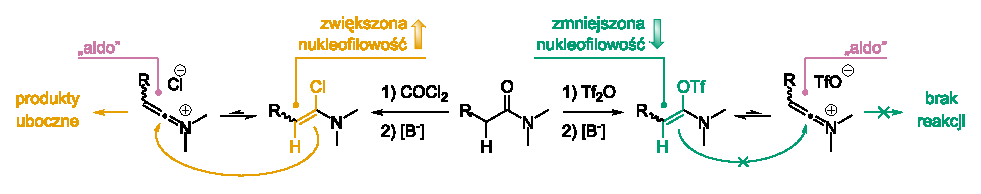
\includegraphics{schemes/chloro-vs-triflic}
  \caption{Różnica w reaktywności chlorowych i triflowych pochodnych enamin z solami ketenimin.
  \label{sch:chloro-vs-triflic}
\end{scheme*}

\section{Amidy Weinreba}


\section{Kalityczna aktywacja kompleksami metali}

\section{Odczynnik Schwartza}

\section{Szerzej o hyrdocyrkonowaniu}

\section{Z własnego podwórka}

\section{Rezonans zakłócony geometrią}